\section{Introduction}


The \lhcb detector is a single-arm forward spectrometer designed 
for precision measurements of particles containing \bquark quarks~\cite{Alves:2008zz}. 
It is one of the four main experiments at the Large Hadron Collider (\lhc) at the 
European Organisation for Nuclear Research (\cern) in Geneva, Switzerland.
In this chapter the \lhcb detector, its performance and its use to select \BdToKstmm events is shown.
The \lhcb detector is described in Section~\ref{sec:lhcb:det} detailing the sub-detector components
 required for measurements of \bsll decays. % (Section~\ref{sec:lhcb:sub}).
The trigger system used in the \lhcb detector is described in Section~\ref{sec:lhcb:trig} and 
an overview of the software used in \lhcb is given in Section~\ref{sec:lhcb:soft}.
The development of the trigger system used to select \BdToKstmm decays for the 2011 data-taking is presented in Section~\ref{sec:lhcb:trigdev} 
along with the final configuration of the \lhcb trigger system used throughout 2011.
%The high performance of the \lhcb detector throughout 2011 is presented in Section~\ref{sec:lhcb:perf}.

\subsection[CERN]{\cern}

\cern is an international organisation founded in 1954 in order to provide a 
politically neutral place to carry out research in nuclear and particle physics.
At the time of writing, \cern has 20 full member states and there are around ten thousand people associated with science at \cern.
Over the years that \cern has operated, it has contributed to the discovery of neutral currents~\cite{Hasert:1973ff}, 
the electroweak gauge bosons~\cite{Arnison:1983rp,Arnison:1983mk} and recently the Higgs boson~\cite{CMS:2012gu,ATLAS:2012gk}.
\cern is primarily home to the \lhc accelerator complex, which is a proton-proton ($pp$) collider with a circumference
 of 27\km at a depth of 100\m under the the French-Swiss border just outside Geneva.
The \lhc accelerator is built in the tunnel originally used for the \lep accelerator and ran at an energy of 
\sqs=7\tev in 2011.
The injection chain  for the \lhc consists of one linear accelerator and three synchrotrons as shown in Fig.~\ref{fig:lhccomplex}. 
\begin{figure}[tbp]
\centering
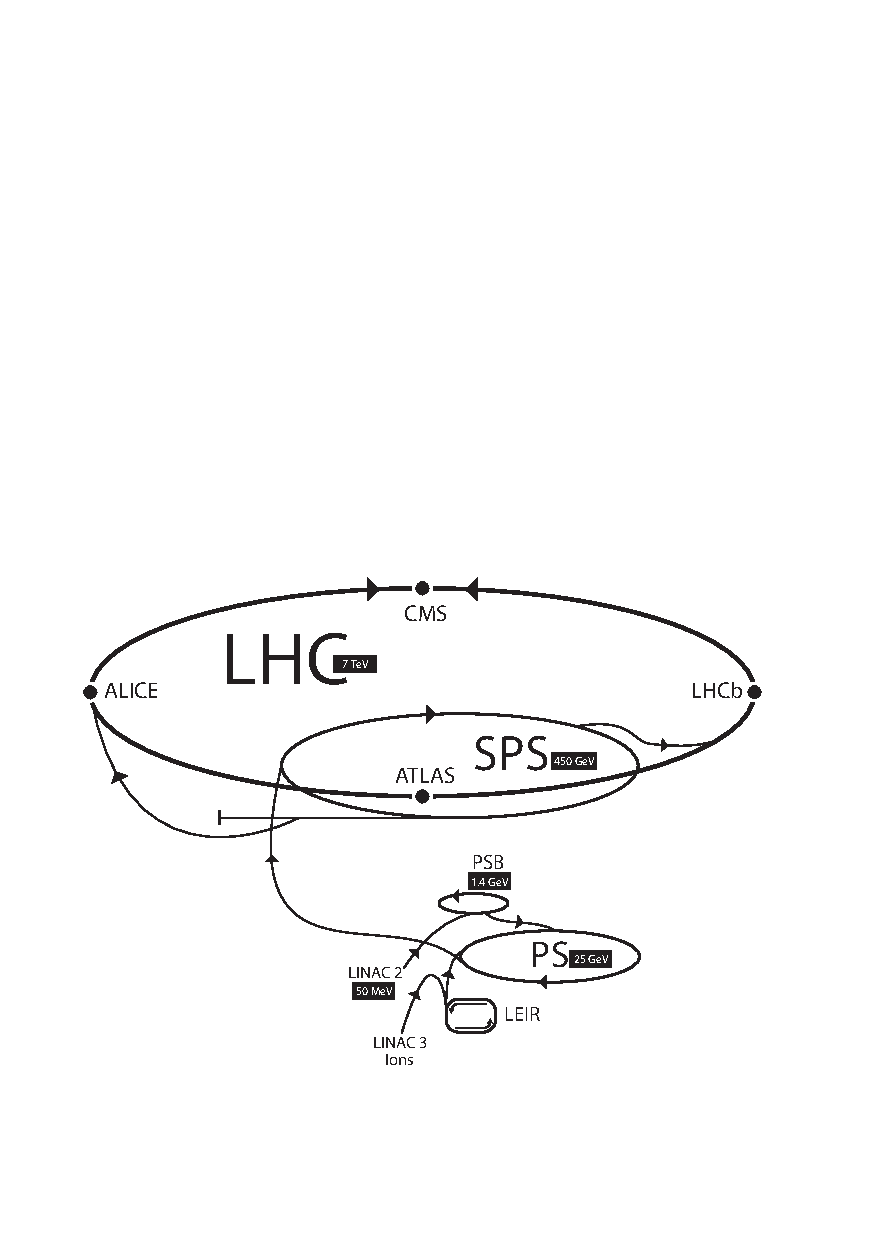
\includegraphics[width=0.48\columnwidth]{chapter3/figs/cern.pdf}
\caption[The \lhc ring.]{A illustration of the the \lhc accelerator complex showing each of the stages in the injection chain 
 for the \lhc ring along with the four main experiments on the \lhc ring~\cite{Lefevre:1092437}. ~\label{fig:lhccomplex} }
\end{figure}
It starts with a linear accelerator which accelerates the protons from rest to 50\mev. 
The synchrotrons increase the beam energy and refine the proton bunches to a configuration suitable for the \lhc. 
Firstly the Proton Synchrotron Booster (PSB) takes the beam from 50\mev to 1.5\gev at which point the 
beam enters the Proton Synchrotron (PS) where the beam energy is increased to 25\gev. 
The beam is then transferred to the Super Proton Synchrotron (SPS) which increases the energy to 450\gev
 before injecting the protons into the \lhc. 
The \lhc accelerates the proton bunches from injection energy at 450\gev to the final collision energy, which was 3.5\tev per beam in 2011 and 4\tev per beam in 2012.
Consolidation upgrades of the \lhc to take place in 2013 and 2014 are expected to increase this collision energy to the design energy of 7\tev per beam.
During operation in 2011-12 there were 1380 proton bunches per beam with a bunch spacing of 50\ns.
There are four main experiments on the \lhc ring, two general purpose detectors (\atlas and \cms), 
along with a heavy-ion experiment (\alice) and a dedicated B-physics experiment (\lhcb).

At the \lhcb interaction point the instantaneous luminosity of the colliding proton bunches 
 is constant at around $\lum\approx3\times10^{32}\cm^2\sec^{-1}$. 
This is significantly below the  \lhc  luminosity, which in 2011 reached over $\lum\approx1\times10^{33}\cm^2\squark^{-1}$.
This luminosity was chosen so that the number of interactions per proton bunch crossing ($\mu$) 
stayed uniform throughout the period of proton collisions for each `fill' of the \lhc.
This ensures that the environment is consistent and has a low multiplicity for reconstruction of \B mesons 
but that there is still a sufficient number of \B meson decays of interest for a given number of collisions.

The production of \bbbar pairs in $pp$ interactions is governed predominantly 
by gluon fusion, $gg\to\bbbar$.
The collision of partons of unequal energy and a momentum boost along the direction of the collision results in \bbbar pairs 
that are produced at small angles to the beam axis.
The angular distribution of \bbbar production is shown in Fig.~\ref{fig:lhcb:bbbar}.
\begin{figure}[tbp]
\centering
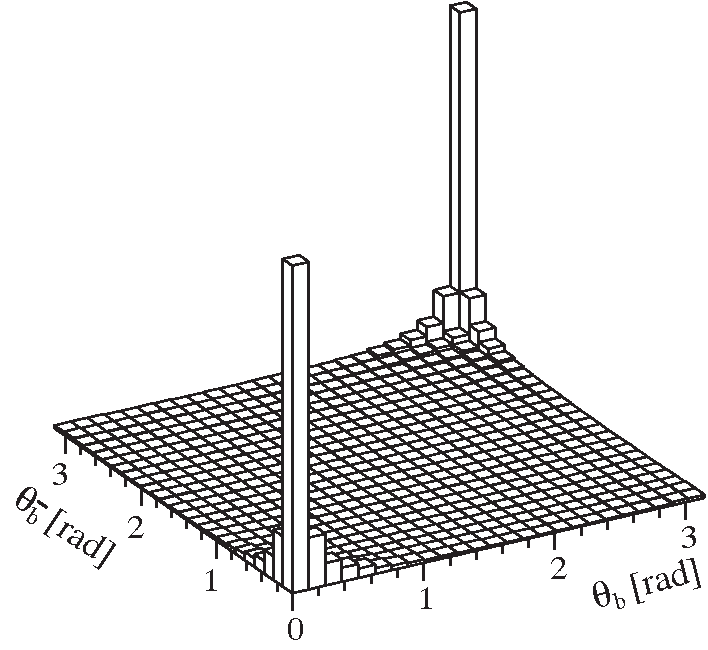
\includegraphics[width=0.48\columnwidth]{chapter3/figs/angular.pdf}
\caption[ $b\bar{b}$ production at the LHC ]{The angular distribution of \bbbar pairs in terms of the polar angle from the beam axis.
The \bbbar pairs are largely produced within a very small opening angle hence the development of \lhcb as a forward spectrometer
~\cite{Alves:2008zz}.~\label{fig:lhcb:bbbar} }
\end{figure}
The \bbbar cross section at \sqs=7\tev is 75\mub within the \lhcb acceptance~\cite{LHCb-PAPER-2010-002}. 
%This corresponds to around $10^7$ \bbbar pairs produced in the 2011 year of data-taking.
In total the experiment recorded an integrated luminosity of 1.0\invfb in 2011 that could be used for further analysis.
The increase in integrated luminosity throughout the year can be seen in Fig.~\ref{fig:lhcb:intlumi} along with the technical stops
 and periods of machine development.
\begin{figure}
\centering
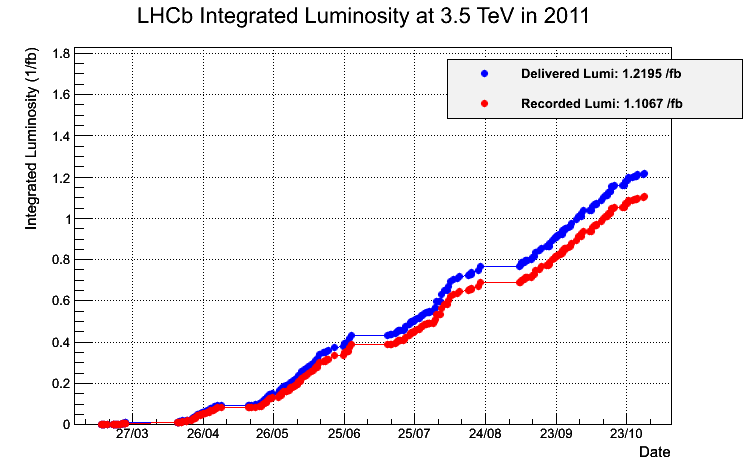
\includegraphics[width=0.66\columnwidth]{chapter3/figs/2011IntegratedLumiLHCbTime_NoPie.png}
\caption{The integrated luminosity recorded by \lhcb during 2011~\cite{OpsPlots}.~\label{fig:lhcb:intlumi} }
\end{figure}
